% Build from docs/reports with bun run pdf labs/07.
\documentclass[11pt]{article}
\newcommand{\sprintname}{Lab 7}
\newcommand{\deliverable}{CPE334 Lab 7, Sprint 1 maintenance and release readiness}
% ---------------------------------------------------------------------------
% Shared preamble of every ClaimFlow sprint report. Build with XeLaTeX from
% the sprint folder (bun run pdf sprint-N). Before \input{../preamble},
% main.tex defines \sprintname (Sprint 1) and \deliverable (Project
% Deliverable 1).
%
% Fonts: Times New Roman and Courier New ship with Windows and macOS and both
% carry the arrows and comparison signs the sources use. A glyph neither has
% shows as "Missing character" in main.log; check-report counts those.
% ---------------------------------------------------------------------------
\usepackage{fontspec}
\setmainfont{Times New Roman}
\setmonofont{Courier New}

% Student names and IDs, from docs/reports/.env through bun run identity.
\InputIfFileExists{build/identity.tex}{}{%
  \errmessage{build/identity.tex is missing: run bun run identity <sprint>}}

\usepackage[a4paper, margin=2cm]{geometry}
\usepackage{graphicx}
\usepackage{pdflscape}
\usepackage{booktabs}
\usepackage{longtable}
\usepackage{array}
\usepackage{xcolor}
\usepackage{fvextra}
\usepackage{float}
\usepackage{caption}
\usepackage{etoolbox}
\usepackage{refcount}
\usepackage{seqsplit}
\usepackage{fancyhdr}

% Colours before hyperref, which reads linkcolor as it loads.
\definecolor{brand}{HTML}{1B5E3F}
\definecolor{todored}{HTML}{C62828}
\usepackage[colorlinks=true, urlcolor=blue!55!black, linkcolor=brand,
            pdftitle={ClaimFlow \sprintname\space report},
            pdfauthor={\studentOneName; \studentTwoName}]{hyperref}

\setlength{\parindent}{0pt}
\setlength{\parskip}{5pt}
\setlength{\emergencystretch}{3em}
\hfuzz=3pt % ignore overfull boxes under 3 pt, which no reader can see
\captionsetup{font=small}
\setcounter{tocdepth}{2}
\setcounter{secnumdepth}{0}

\pagestyle{fancy}
\fancyhf{}
\fancyfoot[L]{\footnotesize ClaimFlow, \sprintname\space report}
\fancyfoot[R]{\footnotesize page \thepage}
\renewcommand{\headrulewidth}{0pt}
\fancypagestyle{plain}{\fancyhf{}\fancyfoot[R]{\footnotesize page \thepage}%
  \renewcommand{\headrulewidth}{0pt}}

% ---- Evidence that is not there yet ---------------------------------------

% Red inline text. check-report counts every \todo and \pending.
\newcommand{\todo}[1]{\textcolor{todored}{\textbf{[TODO: #1]}}}

% A red box where a capture or section is still waiting for something.
% \pending{what it shows}{what it waits for}
\newcommand{\pending}[2]{%
  \par\medskip\noindent\fcolorbox{todored}{white}{\parbox{0.97\linewidth}{%
    \textcolor{todored}{\textbf{[PENDING: #1]}}\\
    \small\itshape Waits for: #2}}\par\medskip}

% ---- Parts -----------------------------------------------------------------

% \reportpart{A}{Title}: starts a page, adds the contents entry, and sets
% part:A:start. \reportpartend{A} sets part:A:end on the last page, so the
% navigation table can print real page ranges with \pageref.
\newcommand{\reportpart}[2]{%
  \clearpage
  \phantomsection
  \addcontentsline{toc}{section}{Part #1: #2}%
  \label{part:#1:start}%
  {\noindent\bfseries\Large\color{brand} Part #1: #2\par}%
  \vspace{2pt}\noindent\textcolor{brand}{\rule{\linewidth}{1.2pt}}\par
  \vspace{6pt}}
\newcommand{\reportpartend}[1]{\par\label{part:#1:end}}
% \pages{A} prints "pp. 5--12" or "p. 5"
\newcommand{\pages}[1]{%
  \ifnumequal{\getpagerefnumber{part:#1:start}}{\getpagerefnumber{part:#1:end}}%
    {p.\ \pageref{part:#1:start}}%
    {pp.\ \pageref{part:#1:start}--\pageref{part:#1:end}}}

% Sub-headings inside a part.
\newcommand{\partsection}[2]{%
  \phantomsection\addcontentsline{toc}{subsection}{#1\ \ #2}%
  \par\bigskip{\noindent\bfseries\large\color{brand} #1\ \ #2\par}\smallskip}

% ---- Evidence figures --------------------------------------------------------

\newcommand{\evidencemaxheight}{22cm}

% The red box drawn when a figure file does not exist, so the build never
% fails on a missing capture.
\newcommand{\figmissing}[2]{%
  \fbox{\parbox[c][3cm][c]{0.94\linewidth}{\centering
    \textcolor{todored}{\textbf{[PENDING FIGURE: \detokenize{#1}]}}\\[4pt]
    \small\itshape #2}}}

% \evidence{figures/x.png}{Caption}: one full-width numbered figure.
\newcommand{\evidence}[2]{%
  \IfFileExists{#1}%
    {\begin{figure}[H]\centering
       \fbox{\includegraphics[width=0.96\linewidth,height=\evidencemaxheight,keepaspectratio]{#1}}%
       \caption{#2}\end{figure}}%
    {\begin{figure}[H]\centering\figmissing{#1}{#2}\caption{#2}\end{figure}}}

% \evidencepart{figures/x-p2.png}{Caption}: one unnumbered piece of a sliced capture.
\newcommand{\evidencepart}[2]{%
  \IfFileExists{#1}%
    {\begin{figure}[H]\centering
       \fbox{\includegraphics[width=0.96\linewidth,height=\evidencemaxheight,keepaspectratio]{#1}}%
       \caption*{\small\itshape #2}\end{figure}}%
    {\begin{figure}[H]\centering\figmissing{#1}{#2}\caption*{\small\itshape #2}\end{figure}}}

% \evidencehalf{file}{caption}: wide capture, at most 11.5 cm tall, two to a page.
\newcommand{\evidencehalf}[2]{%
  \IfFileExists{#1}%
    {\begin{figure}[H]\centering
       \fbox{\includegraphics[width=0.96\linewidth,height=11.5cm,keepaspectratio]{#1}}%
       \caption{#2}\end{figure}}%
    {\begin{figure}[H]\centering\figmissing{#1}{#2}\caption{#2}\end{figure}}}

% \diagramfull{file}{caption}: one Mermaid diagram of a captured document,
% photographed on its own at 3x by scripts/capture-diagrams.ts, at full text width.
\newcommand{\diagramfull}[2]{%
  \IfFileExists{#1}%
    {\begin{figure}[H]\centering
       \fbox{\includegraphics[width=0.96\linewidth,height=\evidencemaxheight,keepaspectratio]{#1}}%
       \caption{#2}\end{figure}}%
    {\begin{figure}[H]\centering\figmissing{#1}{#2}\caption{#2}\end{figure}}}

% \diagramwide{file}{caption}: a diagram much wider than tall, on its own landscape page.
\newcommand{\diagramwide}[2]{%
  \IfFileExists{#1}%
    {\begin{landscape}\begin{figure}[H]\centering
       \fbox{\includegraphics[width=0.96\linewidth,height=15cm,keepaspectratio]{#1}}%
       \caption{#2}\end{figure}\end{landscape}}%
    {\begin{figure}[H]\centering\figmissing{#1}{#2}\caption{#2}\end{figure}}}

% \evidencesmall{file}{caption}{width fraction}: a capture that is small to begin with.
\newcommand{\evidencesmall}[3]{%
  \IfFileExists{#1}%
    {\begin{figure}[H]\centering
       \fbox{\includegraphics[width=#3\linewidth,keepaspectratio]{#1}}%
       \caption{#2}\end{figure}}%
    {\begin{figure}[H]\centering\figmissing{#1}{#2}\caption{#2}\end{figure}}}

% \docsource{docs/srs.md}{sprint-1}{abc1234}: the line above each captured document.
\newcommand{\docsource}[3]{%
  \par\noindent{\small\textbf{Source:} \texttt{\detokenize{#1}} as GitHub renders it,
  captured from \texttt{\detokenize{#2}} at commit \texttt{\detokenize{#3}}.}\par\smallskip}

% ---- Code and terminal output ------------------------------------------------

\DefineVerbatimEnvironment{shell}{Verbatim}
  {fontsize=\footnotesize, frame=single, framesep=5pt, rulecolor=\color{black!25},
   breaklines=true, breaksymbolleft={}}
\DefineVerbatimEnvironment{codeblock}{Verbatim}
  {fontsize=\scriptsize, frame=single, framesep=5pt, rulecolor=\color{black!25},
   breaklines=true, breaksymbolleft={}}

% ---- Title block --------------------------------------------------------------

\newcommand{\reporttitle}{%
  \begin{center}
    {\Large\bfseries CPE 334 --- Introduction to Software Engineering\par}
    \vspace{3pt}
    {\large \deliverable: \sprintname\space report\par}
    \vspace{10pt}
    {\Huge\bfseries\color{brand} ClaimFlow\par}
    {\large Theme 5, Department Expense Reimbursement System\par}
  \end{center}}


\newcolumntype{R}[1]{>{\raggedright\arraybackslash}p{#1}}
\AtBeginEnvironment{longtable}{\small}
\renewcommand{\arraystretch}{1.18}
\DefineVerbatimEnvironment{record}{Verbatim}{fontsize=\footnotesize,
  frame=single, framesep=5pt, rulecolor=\color{black!25},
  breaklines=true, breakanywhere=true, breaksymbolleft={}}
\newcommand{\repo}{https://github.com/beambeambeam/claimflow}
\newcommand{\revision}{\texttt{claimflow-00016-zck}}
\newcommand{\releaseSHA}{\texttt{c32e6455724a0b7be3a5ae8a50889ea50fd4ddbc}}
\newcommand{\runlink}[1]{\href{\repo/actions/runs/#1}{#1}}
\newcommand{\prlink}[1]{\href{\repo/pull/#1}{\##1}}
\newcommand{\issuelink}[1]{\href{\repo/issues/#1}{\##1}}

\begin{document}

\thispagestyle{plain}
\reporttitle

\medskip
\begin{center}
\begin{tabular}{@{}lll@{}}
\toprule
 & \textbf{Student 1} & \textbf{Student 2} \\ \midrule
Name & \studentOneName & \studentTwoName \\
Student ID & \studentOneId & \studentTwoId \\
GitHub & \href{https://github.com/Kiatisakk}{@Kiatisakk} &
  \href{https://github.com/beambeambeam}{@beambeambeam} \\
\bottomrule
\end{tabular}
\end{center}

\begin{longtable}{@{}R{3.8cm}R{12.5cm}@{}}
\toprule
\textbf{Project} & Theme 5, ClaimFlow (Department Expense Reimbursement System). Staff submit claims and the assigned reviewer approves or rejects them. \\
\textbf{Sprint 1 scope} & F-01 Authentication and session, F-02 Submit claim, F-03 My claims, and F-04 Review decision. Lab 7 changes the minimum length of an F-04 rejection reason from 5 to 10 trimmed Unicode code points. \\
\textbf{Repository} & \url{https://github.com/beambeambeam/claimflow} \\
\textbf{Sprint 1 baseline} & \texttt{v0.0.3.0} at \texttt{ac5bce5}, release \prlink{69}. \\
\textbf{Accepted Lab 6} & \texttt{bb5a0d1}, release \prlink{93}, Cloud Run \texttt{claimflow-00010-985}. \\
\textbf{Pre-change version} & \texttt{214d1d5} on \texttt{main}, Cloud Run \texttt{claimflow-00015-vh7}. \\
\textbf{Submitted version} & \href{\repo/releases/tag/v0.1.0.0}{\texttt{v0.1.0.0}} at \releaseSHA{} on \texttt{main}. \\
\textbf{Deployed version} & Same commit at \url{https://claimflow-5bcxewbqkq-as.a.run.app}, revision \revision{}. \\
\textbf{Readiness} & \textbf{READY} for the maintained Sprint 1 scope. Automated gates, public smoke, and authenticated HTTP and browser checks passed. \\
\bottomrule
\end{longtable}

\section*{Seeded users}
\begin{longtable}{@{}R{2.4cm}R{1.9cm}R{3.2cm}R{8.0cm}@{}}
\toprule
\textbf{Username} & \textbf{Role} & \textbf{Position} & \textbf{Can do} \\ \midrule
\texttt{req.anan} & requester & Staff, Section A & Submit claims. \texttt{rev.malee} reviews them. \\
\texttt{req.ploy} & requester & Staff, Section A & Submit claims. \texttt{rev.malee} reviews them. \\
\texttt{req.niran} & requester & Staff, Section B & Submit claims. \texttt{rev.somchai} reviews them. \\
\texttt{rev.malee} & reviewer & Section Head A & Approve or reject claims from \texttt{req.anan} and \texttt{req.ploy}. Submit claims. \texttt{rev.prasert} reviews them. \\
\texttt{rev.somchai} & reviewer & Section Head B & Approve or reject claims from \texttt{req.niran}. Submit claims. \texttt{rev.prasert} reviews them. \\
\texttt{rev.prasert} & reviewer & Department Head & Approve or reject claims from \texttt{rev.malee} and \texttt{rev.somchai}. Submit claims. \texttt{fin.wanida} reviews them. \\
\texttt{fin.wanida} & finance & Finance Officer & Approve or reject claims from \texttt{rev.prasert}. Cannot submit claims. \\
\bottomrule
\end{longtable}

\clearpage
\section*{Contents and evidence}
\begin{longtable}{@{}R{0.8cm}R{2.3cm}R{12.8cm}@{}}
\toprule
\textbf{Part} & \textbf{Pages} & \textbf{Content and evidence IDs} \\ \midrule
A & \pages{A} & Request and baselines (A-01), impact trace and contract revisions (A-02), STS and pre-code review (A-03). \\
B & \pages{B} & Test-first results (B-01, B-02), contract and implementation diffs (B-03), regression (B-04), integration and CI (B-05), deployment, HTTP and browser checks (B-06 to B-08). \\
C & \pages{C} & Five metrics, source records, and one action (C-01 to C-05). \\
D & \pages{D} & Readiness, defects, debt, ownership, retrospective, and disclosures (D-01 to D-03). \\
\bottomrule
\end{longtable}

Times are UTC. The release merged, deployed and was checked on 25 November 2026 in Thailand (ICT, UTC+7). Evidence excerpts contain the information used to assess the report. Links provide access to the original records.


\reportpart{A}{Change impact and revised contract}
\partsection{A-01}{Request, acceptance and baseline}
\label{ev:request}
\issuelink{99} (L7/01), opened by \texttt{beambeambeam} on 22 November 2026 and assigned to \texttt{Kiatisakk}, changes BR-04 under FR-06 as delivered in F-04. A six-character reason such as “No pic” passed the original rule and could leave the requester unsure what to correct. The longer minimum requires more text. The prior minimum conformed to Sprint 1 requirements.

On 23 November at 14:44, \texttt{Kiatisakk} asked for the real RED baseline and the missing SDS, OpenAPI, generated-client and test impacts. \texttt{beambeambeam} recorded the update at 16:16. On 24 November at 16:17:51, \texttt{beambeambeam} recorded in \href{\repo/issues/99\#issuecomment-7137433075}{issue \#99} that the course announcement \emph{Lab 7 Spec Sheet Change} waived instructor and TA approval. The same comment retained teammate review, which \prlink{101} records below. The issue comment is the evidence for the waiver.

\begin{longtable}{@{}R{3.4cm}R{5.4cm}R{7.1cm}@{}}
\toprule
\textbf{Stage} & \textbf{Version} & \textbf{Evidence and relationship} \\ \midrule \endhead
Accepted Sprint 1 & \texttt{v0.0.3.0} / \texttt{ac5bce5} & \prlink{69}, 15 Nov. BR-04 minimum 5. \\
Accepted Lab 6 & \texttt{bb5a0d1} / \texttt{claimflow-00010-985} & \prlink{93}, deployed 21 Nov. Partner accepted on 22 Nov at 11:27 after retesting \#86 and \#87. BR-04 minimum 5. \\
Pre-change code and deploy & \texttt{214d1d5} / \texttt{claimflow-00015-vh7} & 22 Nov. Deploy demo \runlink{45040335622}. BR-04 minimum 5. API RED uses this source. \\
Reviewed contract & \texttt{78fe104}, \texttt{d9feee9}, squash \texttt{124cf9a} & \prlink{101}, merged into \texttt{lab-7} on 24 Nov. See A-03 on p.~\pageref{ev:contract-review}. \\
OpenAPI, RED, GREEN & \texttt{ea1537b}, then \texttt{405c906}, \texttt{6cabc3e}, \texttt{b51c058}, \texttt{0226536} & 24 Nov. OpenAPI schema, separate test commits, then implementation and a Playwright locator fix. See B-01 on p.~\pageref{ev:redgreen}. \\
Staging and main & \texttt{8b660a1} then \texttt{c32e645} / \texttt{v0.1.0.0} & \prlink{105} into \texttt{lab-7}, then \prlink{106} into \texttt{main}. Same tree as approved implementation head \texttt{9b1fc9c}. See B-05 on p.~\pageref{ev:release}. \\
Deployed main & \texttt{c32e645} / \revision{} & Deploy demo \runlink{45453647851}, 24 Nov. Deployment and smoke evidence in B-06 on p.~\pageref{ev:deploy}. \\
\bottomrule
\end{longtable}

Between Lab 6 and the pre-change baseline, \#94, \#95, \#96 and \#98 updated documentation. Sprint 1 follow-ups \prlink{97} (\texttt{fbf4382}) changed 43 app files, including F-04's decision panel, contract reader, generated schema and test. The counter began reading the contract limit and a decision 403 opened the access page. The API minimum remained 5 in all three baselines.

\clearpage
\partsection{A-02}{Impact and versioned contract}
\label{ev:impact}
\begin{longtable}{@{}R{2.8cm}R{4.2cm}R{3.8cm}R{5.0cm}@{}}
\toprule
\textbf{Requirement / feature} & \textbf{Contract sections} & \textbf{AC / STS} & \textbf{Code and dependency} \\ \midrule \endhead
BR-04 and NFR-08 / F-04 &
SRS \S7 BR-04 and F-04 \S\S1.5, 1.6, 2.2 revised. SDS \S2.2 history comment revised. SRS \S8 and SDS \S4.2 field error structure preserved. &
F04-AC-06, 18 and F04-TEST-06, 07, 21, 24 revised. &
\texttt{rules.go}, \texttt{openapi.yaml}, \texttt{openapi-ts.config.ts}, generated clients, \texttt{contract.ts}, \texttt{decision-panel.tsx}. API callers must send 10 or more for reject. \\
FR-06, FR-07 / F-04, F-03 &
SRS \S6, F-04 \S\S1.3, 1.4 and 3 (decision, order, HTTP), SDS \S\S3.2, 3.3 unchanged. &
F04-AC-05. F04-TEST-05, 23 and the existing success path in 24. &
\texttt{handler.go} and \texttt{service.go} preserve the decision and history read. Approval comment remains optional, with max 500. \\
BR-01, 02, 03, 11, 13 and NFR-06 / F-04 &
F-04 \S\S1.4, 3. SDS \S\S2.2, 3.3, 5.2. &
F04-AC-07 to 15. F04-TEST-08 to 18. &
Only the assigned reviewer may decide and never their own claim. State, version, history transaction and access precedence stay in the service and handlers. \\
BR-04 / later F-06 and F-08 &
SRS \S7 sets the new minimum for return and final reject. &
F06-AC-02 and F06-TEST-02/03 are planned in \prlink{100}. &
Return and final reject fall outside this implementation. \\
\bottomrule
\end{longtable}

\textbf{Data and configuration.}
\texttt{claim\_history.comment} is nullable \texttt{VARCHAR(500)} with no minimum-length constraint. BR-04 runs on new writes, before the conditional update and history insertion. Under BR-11, history is append-only and 5--9 character historical reasons stay readable as stored. No data backfill, schema migration or new configuration is needed. ADR-0001 covers reviewer assignment and remains applicable.

\textbf{Old and revised specification excerpts.}
Part A revised SRS 0.2 to 0.3, F-04 0.7 to 0.8, System SDS 0.17 to 0.18, and the traceability change log dated 24 November.
\begin{longtable}{@{}R{3.1cm}R{6.4cm}R{6.4cm}@{}}
\toprule
\textbf{Section} & \textbf{Old} & \textbf{Revised} \\ \midrule \endhead
SRS \S7 BR-04 & Reject, return and final reject need a non-blank comment of 5--500 characters. Approve may include an optional comment. & Reject, return and final reject need a non-blank comment of 10--500 characters. Approve may include an optional comment. \\
System SDS \S2.2 & History comment is nullable, required at 5--500 non-blank characters for REJECT, RETURN and FINAL\_REJECT, checked by the claim module. & Required at 10--500 non-blank characters on write for those actions. Entries under the former minimum are kept as stored under BR-11. \\
F-04 \S2.2 and AC-18 (Reject control) & Required reason, counter, field messages and Reject and Cancel controls. & Keep Reject disabled below 10 after trimming. Show the minimum-length message once text is entered. Use API metadata for limits and display API 422 field errors. \\
\bottomrule
\end{longtable}

\clearpage
\partsection{A-03}{Acceptance criteria, STS and contract review}
\label{ev:contract-review}
\textbf{F-04 \S\S1.5--1.6 and F04-AC-06.}
For \texttt{POST /claims/\{id\}/reject}, the assigned reviewer acts on a \texttt{SUBMITTED} claim using its current \texttt{If-Match} version. The prior boundary row was 4 / 5 / 500 / 501 characters. The revised row is 9 / 10 / 500 / 501. Both rows expect 422 / 200 / 200 / 422 respectively. Count Unicode code points after trimming edge whitespace.

\begin{longtable}{@{}R{3.1cm}R{6.4cm}R{6.4cm}@{}}
\toprule
\textbf{Case} & \textbf{Old outcome} & \textbf{Revised outcome} \\ \midrule \endhead
Missing or blank & 422, “Enter a reason (5 to 500 characters).” & 422, “Enter a reason (10 to 500 characters).” \\
1--4 characters & 422, “Reason must be at least 5 characters.” & 422, “Reason must be at least 10 characters.” \\
5--9 characters & 200, \texttt{REJECTED}. & 422, “Reason must be at least 10 characters.” \\
10--500 characters & 200, \texttt{REJECTED}. & 200, \texttt{REJECTED}. \\
501 characters & 422, “Comment cannot be more than 500 characters.” & Same 422 and message for reject or approve. \\
\bottomrule
\end{longtable}
All these 422s identify field \texttt{comment} and rule \texttt{BR-04}. A 422 leaves status, version and history intact. Authentication, access, missing claim, transition, and version checks keep their prior conditions and precedence. F04-AC-05 preserves stored rejection reason and requester history.

\textbf{Revised STS cases.}
\begin{longtable}{@{}R{3.3cm}R{12.8cm}@{}}
\toprule
\textbf{Test / criterion} & \textbf{Preconditions, input and expected result} \\ \midrule \endhead
F04-TEST-06 \newline Module / AC-06 & Act as assigned reviewer on a submitted claim. Missing, blank, 9 (was 4), and 501 fail with one matching \texttt{ValidationError}. 10 (was 5) and 500 succeed. Trimmed and Thai-character cases enforce character count. Approve accepts no comment or up to 500 and rejects 501. Compare stored state after refusal. \\
F04-TEST-07 \newline HTTP / AC-06 & Same role, state and current version. Missing body, missing comment, empty, blanks, 9 (was 4), and 501 give exact 422 field errors and preserve state. 10 and 500 reject successfully. Approve with 501 gives 422. \\
F04-TEST-21 \newline Component / AC-18 & Open Reject for a submitted claim. Empty and trimmed 9 block submission. At 10 the control enables, including Unicode vectors. A valid-length “No receipt” (was “No”) reaches the mocked 422. Keep input and show API error. Retain success, 409 and 403 checks. \\
F04-TEST-24 \newline E2E / AC-05, 18 & Seed requester and assigned reviewer. Submit a claim, open it from the reviewer queue, check disabled for empty and “No photos” (9), and check its message. Submit “Receipt missing” (15) as before. Requester sees Rejected and the reason in history. \\
\bottomrule
\end{longtable}

\textbf{Pre-implementation review.}
In \prlink{101}, \texttt{beambeambeam} reviewed \texttt{d8077b2} on 24 November at 12:22. Findings covered the unreachable mocked 422, missing disabled-control steps, stale pass labels, the generator hook and OpenAPI review order. \texttt{Kiatisakk} updated \texttt{d9feee9}. The \href{\repo/pull/101\#pullrequestreview-6043052471}{16:16:11 approval} verified the corrected cases and traceability and requested OpenAPI review before implementation. The approval preceded the 16:18 staging merge and the tests and code in Part B. The OpenAPI review itself came after implementation, as B-05 records.

\reportpartend{A}

\reportpart{B}{Implementation and regression-safe delivery}
\partsection{B-01}{API tests on the old and new rule}
\label{ev:redgreen}
On 24 November, the team captured RED on \texttt{214d1d5} with the revised tests from \texttt{405c906} (service) and \texttt{6cabc3e} (HTTP). GREEN ran those same tests on \texttt{b51c058}. Exact test start times were unavailable.

\textbf{Setup and assertions.}
In \texttt{apps/api/internal/claim/act\_test.go}, F04-TEST-06 creates a PostgreSQL-backed submitted claim per case. Its assigned reviewer calls \texttt{Act} with the current version. A failed decision must give exactly one \texttt{comment}/BR-04 error and leave the claim submitted at its original version, with no decision time and one history entry. Success stores the trimmed reason.

In \texttt{apps/api/claims\_review\_test.go}, F04-TEST-07 logs in as the assigned reviewer on a newly submitted claim. Each 422 must return the expected message and leave the database state equal to the initial snapshot. Each accepted length uses a fresh claim. Selected test body from the 422 loop:
\begin{record}
recorder := decide(t, router, token, id, tc.action, "\"0\"", tc.body)
decodeProblem(t, recorder, http.StatusUnprocessableEntity, "VALIDATION_FAILED")

want := []fieldError{{Field: "comment", Rule: "BR-04", Message: tc.message}}
if got := problemErrors(t, recorder); !slices.Equal(got, want) {
    t.Fatalf("errors = %+v, want %+v", got, want)
}

if after := readState(t, pool, id); after != before {
    t.Fatalf("stored = %+v after the refused decision, want %+v", after, before)
}
\end{record}

\textbf{Commands and captured output.}
Both commands ran from \texttt{apps/api} on RED and GREEN.
\begin{record}
go test -v -count=1 ./internal/claim -run '^TestF04TEST06CommentRuleBR04$'
go test -v -count=1 . -run '^TestF04TEST07CommentRuleIs422WithTheFieldError$'
\end{record}
\begin{record}
RED (exit 1 for both commands)
=== RUN   TestF04TEST06CommentRuleBR04/reject_with_9_characters
    act_test.go:87: Act error = <nil>, want a ValidationError with one field
--- FAIL: TestF04TEST06CommentRuleBR04
=== RUN   TestF04TEST07CommentRuleIs422WithTheFieldError/reject_with_9_characters
    claims_review_test.go:483: status = 200, want 422
--- FAIL: TestF04TEST07CommentRuleIs422WithTheFieldError

GREEN (exit 0 for both commands)
--- PASS: TestF04TEST06CommentRuleBR04
    --- PASS: TestF04TEST06CommentRuleBR04/reject_with_9_characters
    --- PASS: TestF04TEST06CommentRuleBR04/reject_with_10_characters
--- PASS: TestF04TEST07CommentRuleIs422WithTheFieldError
    --- PASS: TestF04TEST07CommentRuleIs422WithTheFieldError/reject_with_9_characters
    --- PASS: TestF04TEST07CommentRuleIs422WithTheFieldError/reject_with_10_characters
\end{record}
RED had 11 pass / 5 fail in the module and 4 pass / 5 fail at HTTP. Old code accepted the 9-character input and used the old blank-reason message. GREEN had 16 module and 9 HTTP passes, 0 failures and 0 skips. GREEN also accepted 500, rejected 501, and preserved state on each 422.

\clearpage
\partsection{B-02}{Dialog and seeded test evidence}
\label{ev:web}
\textbf{F04-TEST-21 (component).}
With a submitted claim and a mocked decision endpoint, the test types a padded 9-character reason and checks the message, disabled state and absence of a POST. It checks Unicode 9/10 cases with edge whitespace, and an empty field. A separate mock returns 422 for “No receipt” (10) to verify API field errors and input retention.
\begin{record}
bun run test run src/features/reviews/__test__/decision-panel.test.tsx
\end{record}
Ran in \texttt{apps/web} on 24 November. At \texttt{6cabc3e}, the short-reason test expected \texttt{ariaDisabled} to be \texttt{"true"} and received \texttt{null}. Counts were 13 passed, 1 failed, 0 skipped. At \texttt{b51c058}, all 14 passed with 0 failed and 0 skipped. The teammate's rerun matched these counts.

\textbf{F04-TEST-24 (Chromium E2E).}
The requester submits a new claim and the assigned reviewer opens it from the queue. The test checks empty and 9-character disabling, submits a valid reason, and opens the claim again as the requester to confirm the transition and stored reason. The paired F04-TEST-23 checks approval and requester history.
\begin{record}
bun run e2e e2e/f04-review-decision.spec.ts
\end{record}
Ran from \texttt{apps/web} on 24 November against local PostgreSQL 17 with seven seeded users and six sample claims. On the RED dialog and spec from \texttt{6cabc3e} with the updated API, the empty-reason check showed \texttt{Expected: disabled} and \texttt{Received: enabled}. This isolates the old dialog. The record gives one failing case. The full RED run totals are unavailable. On \texttt{0226536} with API \texttt{b51c058}, both journeys passed (2 passed, 0 failed, 0 skipped). The follow-up narrowed the Playwright locator to the reason field's accessible description.

\partsection{B-03}{OpenAPI contract and implementation diff}
\label{ev:diff}
The schema edit in \texttt{ea1537b} changed the reject endpoint description and shared \texttt{ClaimDecision.comment} description to 10--500 after trimming. The service returns a 422 with the field error. The shared schema gained metadata while approve kept its optional comment:
\begin{record}
+          x-min-length: 10
           x-max-length: 500
\end{record}
Selected actual lines from the \texttt{b51c058} diff in \texttt{apps/api/internal/claim/rules.go}. The existing trimmed rune count applies before these branches.
\begin{record}
-   MinReasonLength  = 5
+   MinReasonLength  = 10
    MaxCommentLength = 500

    case action == ActionReject && length == 0:
-       message = "Enter a reason (5 to 500 characters)."
+       message = fmt.Sprintf("Enter a reason (%d to %d characters).", MinReasonLength, MaxCommentLength)
    case action == ActionReject && length < MinReasonLength:
-       message = "Reason must be at least 5 characters."
+       message = fmt.Sprintf("Reason must be at least %d characters.", MinReasonLength)
\end{record}

\clearpage
\textbf{B-03 continued.}
The web generator propagates \texttt{x-min-length} into Zod metadata, and \texttt{contract.ts} reads it. Selected actual lines from \texttt{decision-panel.tsx} at \texttt{b51c058} show the reject-only gate and field error:
\begin{record}
+const commentSchema = zClaimDecision.shape.comment.unwrap();
+const reasonMinimum = contractMinLength(commentSchema);
+const commentLimit = contractMaxLength(commentSchema);

+  const reasonTooShort =
+    decision === "reject" &&
+    (comment
+      .replaceAll(
+        /^\p{White_Space}+|(?<!\p{White_Space})\p{White_Space}+$/gu,
+        ""
+      )
+      .match(/./gsu)?.length ?? 0) < reasonMinimum;
+
+  const minimumError =
+    reasonTooShort && comment !== ""
+      ? `Reason must be at least ${reasonMinimum} characters.`
+      : undefined;

+  const commentError = minimumError ?? serverCommentError;
-                isDisabled={send.isPending}
+                isDisabled={send.isPending || reasonTooShort}
\end{record}
Generated outputs changed in \texttt{api.gen.go}, \texttt{types.gen.ts}, \texttt{sdk.gen.ts}, \texttt{react-query.gen.ts} and \texttt{zod.gen.ts}. Generation left a clean diff. The implementation uses the existing write path, permissions, \texttt{If-Match} checks and transaction. No migration or history rewrite was added.

\partsection{B-04}{Regression selection and results}
\label{ev:regression}
The 24 November regression set exercises F-04 dependents. F04-TEST-05 checks the reason in requester history. F04-TEST-08 to 13 cover owner and reviewer access. F04-TEST-14 to 18 cover status, stale and concurrent decisions, rollback and append-only history. F04-TEST-23 covers approval. The web suite also covers the review queue, session and decision errors. Revised expectations are listed in A-03 on p.~\pageref{ev:contract-review}.
\begin{longtable}{@{}R{10.4cm}R{5.7cm}@{}}
\toprule
\textbf{Command and version} & \textbf{Actual result} \\ \midrule \endhead
\texttt{go test -v -count=1 . ./internal/claim -run '\string^TestF04TEST'} at \texttt{b51c058} and \texttt{go test -v -count=1 ./migrations -run '\string^TestF04TEST'} at \texttt{0226536}, both in \texttt{apps/api}. &
19 named F-04 tests passed. No failures or skips reported for this selection. \\
\texttt{bun run test:coverage} in \texttt{apps/api} at \texttt{b51c058}. &
All thresholds passed, 100\% (785/785). The local record gives coverage only. See B-05 for release counts. \\
\texttt{bun run test:coverage --maxWorkers=2 --retry=2} in \texttt{apps/web} at \texttt{0226536}. &
139 passed in 17 files. Statement, branch, function and line coverage were 100\%. Earlier concurrent F01-TEST-20 runs hit login timeouts. \\
Local seeded F-04 E2E at \texttt{0226536} (command and setup in B-02). &
2 passed, 0 failed, 0 skipped. \\
\texttt{bun run generate} and \texttt{bun run vuln} at \texttt{b51c058}. &
Generation left no diff. API scan found no vulnerabilities. \\
\bottomrule
\end{longtable}

\clearpage
\partsection{B-05}{Review, staging and released main}
\label{ev:release}
\begin{longtable}{@{}R{3.8cm}R{12.3cm}@{}}
\toprule
\textbf{24 Nov 2026 (UTC)} & \textbf{Recorded action and review evidence} \\ \midrule \endhead
16:16--16:18 & Contract \prlink{101} approved, then squashed to \texttt{lab-7} as \texttt{124cf9a}. See A-03. \\
16:20--16:28 & OpenAPI contract commit \texttt{ea1537b} came first. Test commits \texttt{405c906} and \texttt{6cabc3e} preceded code \texttt{b51c058}. Implementation proceeded at the maintainer's direction while OpenAPI teammate review was pending. \\
17:16:23 & On \texttt{3e4b572}, \texttt{Kiatisakk} \href{\repo/pull/105\#pullrequestreview-6043999986}{confirmed the OpenAPI diff matched F-04}. The reviewer checked metadata generation, API RED/GREEN, and 50 focused web tests. Requested changes were to record the late review and list RED/GREEN versions per test. The reviewer relied on CI and the PR for full gates and E2E. \\
17:20--17:31 & \texttt{4993321} documented the review. \texttt{9b1fc9c} listed each test's versions. \texttt{Kiatisakk} approved at 17:28:21 after a docs-only follow-up and confirmed the component counts. \prlink{105} squashed to \texttt{lab-7} as \texttt{8b660a1} at 17:31:06. \\
17:47--17:48 & \texttt{Kiatisakk} approved \prlink{106} at 17:47:07 after checking the branch contents, generated rule, and required CI. The reviewer left the four authenticated checks for after deploy. \prlink{106} merged to \texttt{main} at 17:48:05. \issuelink{99} closed as completed at 17:48:07. \\
17:53:02 & Semantic-release published \texttt{v0.1.0.0}. Remote \texttt{main} and that tag both resolved to \releaseSHA{}. \\
\bottomrule
\end{longtable}
The release review calls \texttt{871d373} an approved head. Git identifies it as the tree ID shared by the actual approved \prlink{105} head \texttt{9b1fc9c}, staging squash \texttt{8b660a1} and release merge \texttt{c32e645}. The release's first parent is \texttt{214d1d5} and its second parent is \texttt{8b660a1}. This preserves the \texttt{feat!:} release signal. The 19 changed files cover L7/01 only. The separate Sprint 2 contract PR \#100 and release path \#102 are outside this change.

\textbf{CI.}
The five required jobs (\texttt{api}, \texttt{test}, \texttt{code\_quality}, \texttt{image}, \texttt{build}) passed on \prlink{101} run \runlink{45434761904}, \prlink{105} run \runlink{45447692201}, and \prlink{106} run \runlink{45449479661}. The release job was skipped on PRs. On main run \runlink{45452555188}, all five jobs and the release job succeeded. The release CI ran at \texttt{c32e645}, from 17:48:08 to 17:54:08.

Selected main CI output, with ANSI formatting and runner prefixes removed:
\begin{record}
api   17:52:19  DONE 300 tests in 57.660s
api   17:52:28  Total test coverage: 100% (785/785)
api   17:52:35  No vulnerabilities found.
test  17:48:50  Test Files  17 passed (17)
test  17:48:50  Tests       139 passed (139)
\end{record}
The Go job ran \texttt{gotestsum} with \texttt{-race -coverpkg=./... -coverprofile=coverage.out ./...} in \texttt{apps/api}. Its JUnit artifact (14949441476) confirms 300 passed, 0 failed, 0 errors and 0 skips. The web job ran \texttt{bun run test:coverage} in \texttt{apps/web}, with text-summary, Cobertura, and JUnit outputs. It recorded 0 failures and 0 skips. Local Playwright was run separately, per \prlink{96}.

\clearpage
\partsection{B-06}{Cloud Run deployment and public smoke}
\label{ev:deploy}
Deploy demo \runlink{45453647851} succeeded on 24 November from 17:54:12 to 17:56:06 after the main CI pass. It built from \releaseSHA{}, ran the existing migrate-and-seed job, and deployed by digest to \revision{}. The deployment step reported 100\% traffic to that revision. The digest was:
\begin{record}
sha256:4648f547d5250c04c9240a2b8b4ffe18a3fb4c0cf90501f949d13263f55dcb7e
\end{record}

The workflow ran \texttt{bash deploy/smoke.sh} with the public service URL and expected full SHA. Selected output from 17:55:49--17:55:59:
\begin{record}
Service [claimflow] revision [claimflow-00016-zck] has been deployed and is serving 100 percent of traffic.
PASS /api/v1/health reports c32e6455724a0b7be3a5ae8a50889ea50fd4ddbc
PASS /api/v1/ready 200
PASS / serves the web build
PASS unknown /api route is a JSON 404
\end{record}
The report session reran this read-only smoke from the release checkout against the public URL at about 18:23 UTC. All four checks passed again and the script exited 0.

\partsection{B-07}{Authenticated post-deployment checks}
\label{ev:live}
Automated HTTP probe run on demand against the demo on 24 November, 18:25:50--18:26:14 UTC (25 November, 01:25--01:26 ICT). The input was one fresh synthetic claim, \texttt{CLM-2026-000023}, created with a 250.00 THB travel item. Three role-specific logins returned 200. Creation returned 201. The assigned reviewer read \texttt{SUBMITTED}, ETag \texttt{"0"}, and history \texttt{[SUBMIT]}.

Each attempt called \texttt{POST /api/v1/claims/\{id\}/reject} with \texttt{If-Match: "0"}. After each refused request, an owner read compared status, version, decision time and history with the initial record. Public health reported \texttt{c32e645} before and after the verified run on \revision{}.

\begin{longtable}{@{}R{4.2cm}R{4.8cm}R{7.1cm}@{}}
\toprule
\textbf{Actor and input} & \textbf{Expected result} & \textbf{Actual result at 18:26:13 UTC} \\ \midrule \endhead
Owner \texttt{req.anan}, \texttt{abcdefghij} (10) & 403, no claim data or state change. & \textbf{PASS}. 403 \texttt{FORBIDDEN}, problem fields only, unchanged. \\
Unassigned reviewer \texttt{rev.somchai}, \texttt{abcdefghij} (10) & 403, no claim data or state change. & \textbf{PASS}. 403 \texttt{FORBIDDEN}, problem fields only, unchanged. \\
Assigned reviewer \texttt{rev.malee}, \texttt{abcdefghi} (9) & 422 on \texttt{comment}, BR-04. No state change. & \textbf{PASS}. 422 \texttt{VALIDATION\_FAILED}, field \texttt{comment}, rule BR-04, “Reason must be at least 10 characters.” ETag stayed \texttt{"0"}. \\
Assigned reviewer \texttt{rev.malee}, \texttt{abcdefghij} (10) & 200, \texttt{REJECTED}, version +1, one new history entry. & \textbf{PASS}. 200. Owner reread 200, ETag \texttt{"1"}, \texttt{REJECTED}, history \texttt{[SUBMIT, REJECT]} with reason \texttt{abcdefghij} and assigned reviewer as actor. \\
\bottomrule
\end{longtable}
The first attempt stopped after the owner 403 because the probe treated the standard problem \texttt{instance} request path as returned claim data. The corrected assertion checked the \texttt{instance} echo separately and confirmed the remaining fields contain no claim data. The rerun reused the same claim, finished with 4 passes, 0 failures and 0 skips, and ended all three sessions with 204. The synthetic rejection remains in append-only demo history.

\clearpage
\partsection{B-08}{Live browser checks}
\label{ev:browser}
\textbf{Manual browser walkthrough.}
The report session exercised the deployed web UI on 24 November 2026 at 18:35--18:36 UTC (25 November, 01:35--01:36 ICT). The version page reported \texttt{c32e645}, matching the full SHA for \revision{} in B-06 on p.~\pageref{ev:deploy}. The requester \texttt{req.anan} submitted a fresh synthetic 250.00 THB travel claim, \texttt{CLM-2026-000024}, assigned to \texttt{rev.malee}.

The owner opened the submitted claim and saw its details without Approve or Reject controls. The unassigned reviewer \texttt{rev.somchai} opened the same claim URL and got 403 from the claim detail request. The UI displayed the access denial without showing the claim. Both checks passed before any decision was made.

\begin{figure}[H]
  \centering
  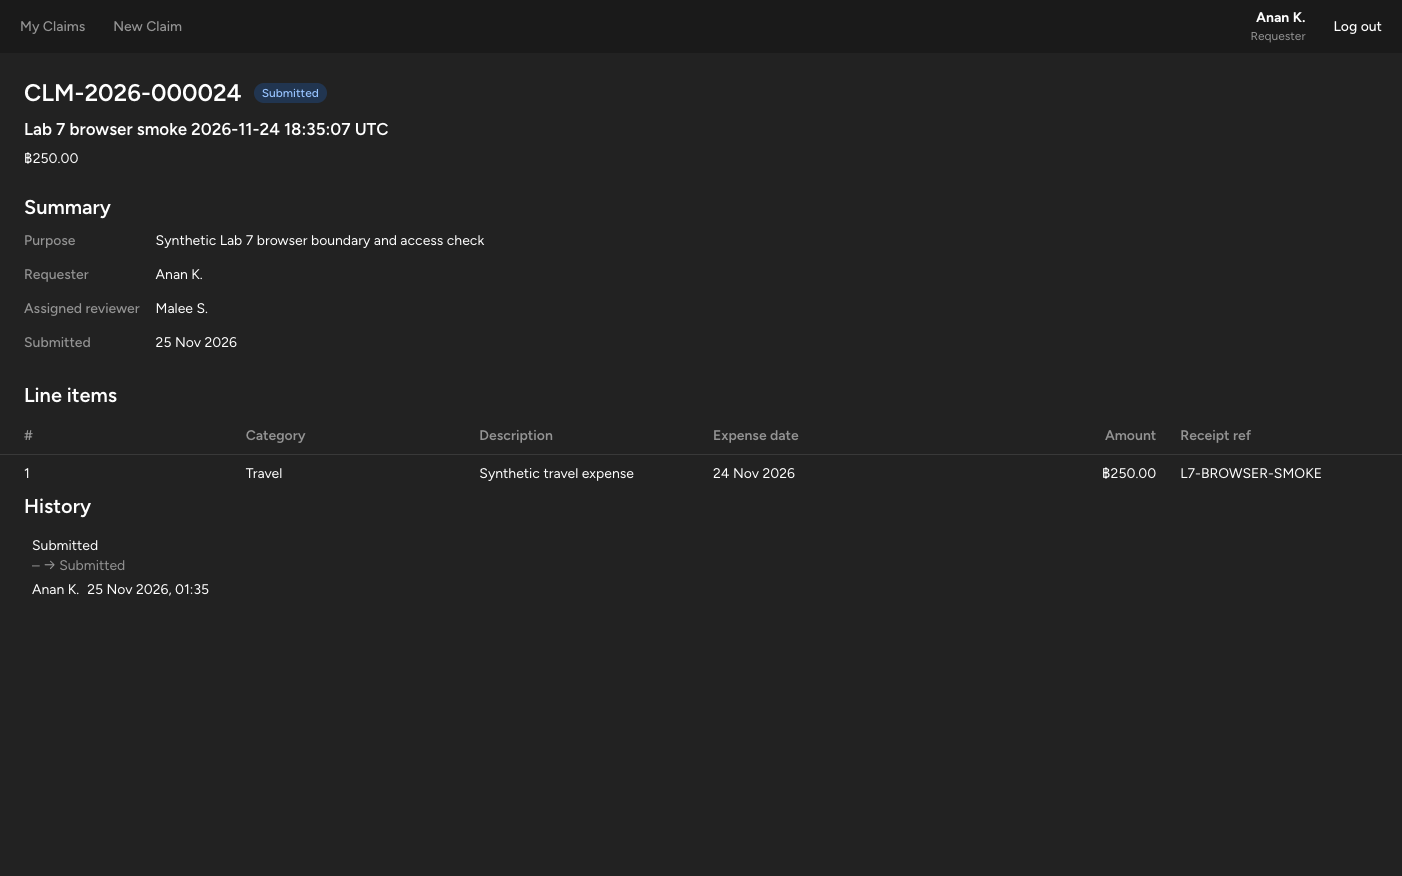
\includegraphics[width=0.96\linewidth,trim=0bp 250bp 0bp 0bp,clip]{figures/deploy/01-owner-submitted.png}
  \caption*{\textbf{B-08a.} The owner can read the submitted claim. The decision controls are absent.}
\end{figure}

\begin{figure}[H]
  \centering
  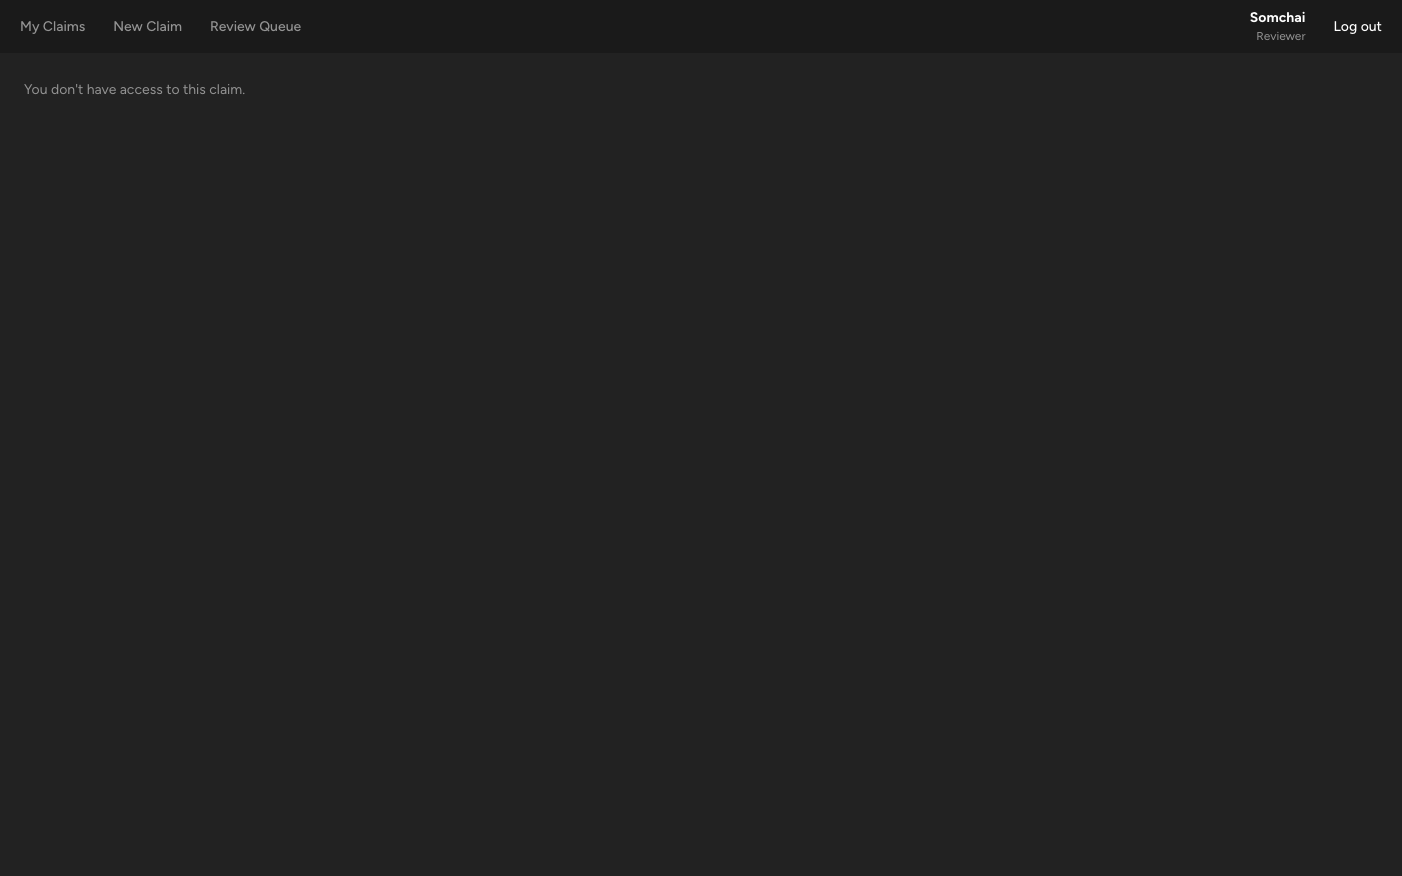
\includegraphics[width=0.96\linewidth,trim=0bp 751bp 0bp 0bp,clip]{figures/deploy/02-unassigned-reviewer.png}
  \caption*{\textbf{B-08b.} Somchai opened the same claim URL. The server returned 403 and the page displayed the denial.}
\end{figure}

\clearpage
\textbf{B-08 continued.}
Malee opened the claim from the Review Queue. An empty reason disabled Reject. Typing “No photos” showed the minimum-length message and left Reject disabled at 9. Replacing it with “No receipt” removed the inline error and enabled Reject at 10. Clicking Reject returned HTTP 200 at 18:36:27 UTC.

\begin{figure}[H]
  \centering
  \begin{minipage}[t]{0.48\linewidth}
    \centering
    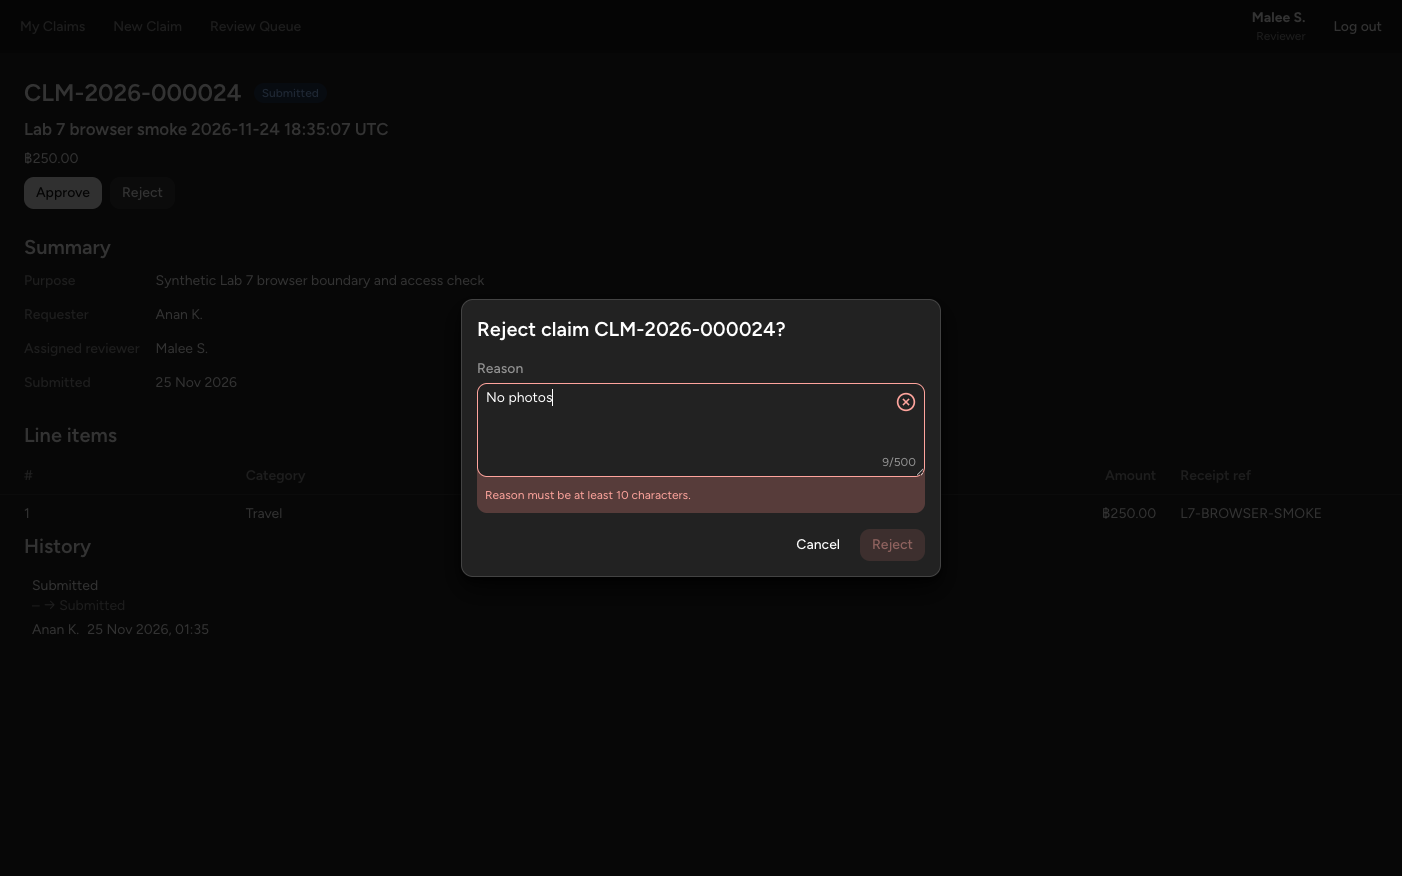
\includegraphics[width=\linewidth,trim=447bp 284bp 447bp 288bp,clip]{figures/deploy/03-reason-9.png}
    \caption*{\textbf{B-08c.} Nine characters. Reject is disabled and the field shows the minimum-length message.}
  \end{minipage}\hfill
  \begin{minipage}[t]{0.48\linewidth}
    \centering
    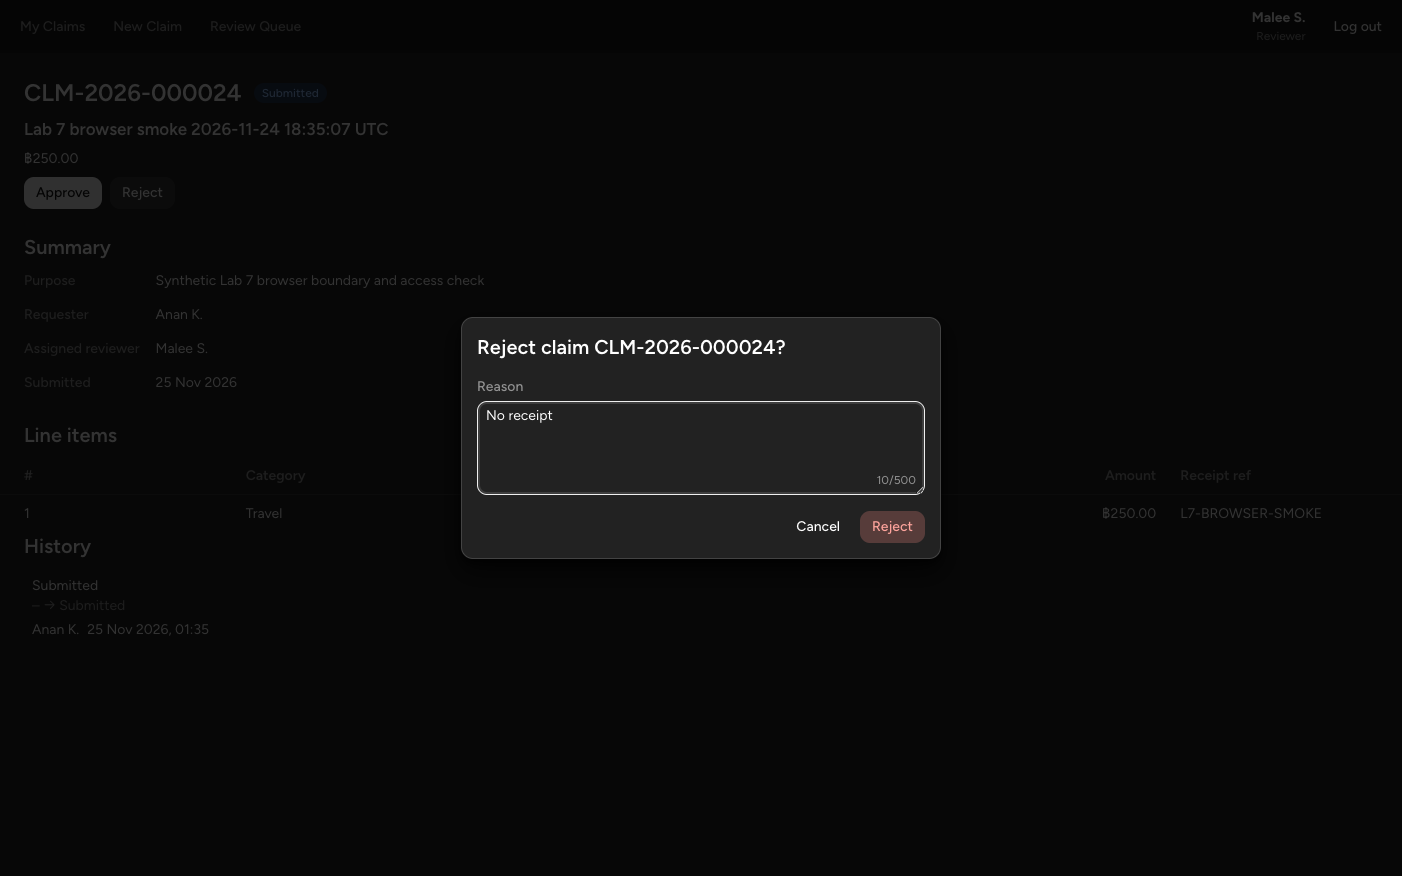
\includegraphics[width=\linewidth,trim=447bp 284bp 447bp 288bp,clip]{figures/deploy/04-reason-10.png}
    \caption*{\textbf{B-08d.} Ten characters. Reject is enabled and the inline error clears.}
  \end{minipage}
\end{figure}

The requester signed back in and opened the claim from My Claims. The status was Rejected and the history showed Malee's decision with the stored reason. All six browser checks passed. The synthetic claim remains in demo history.

\begin{figure}[H]
  \centering
  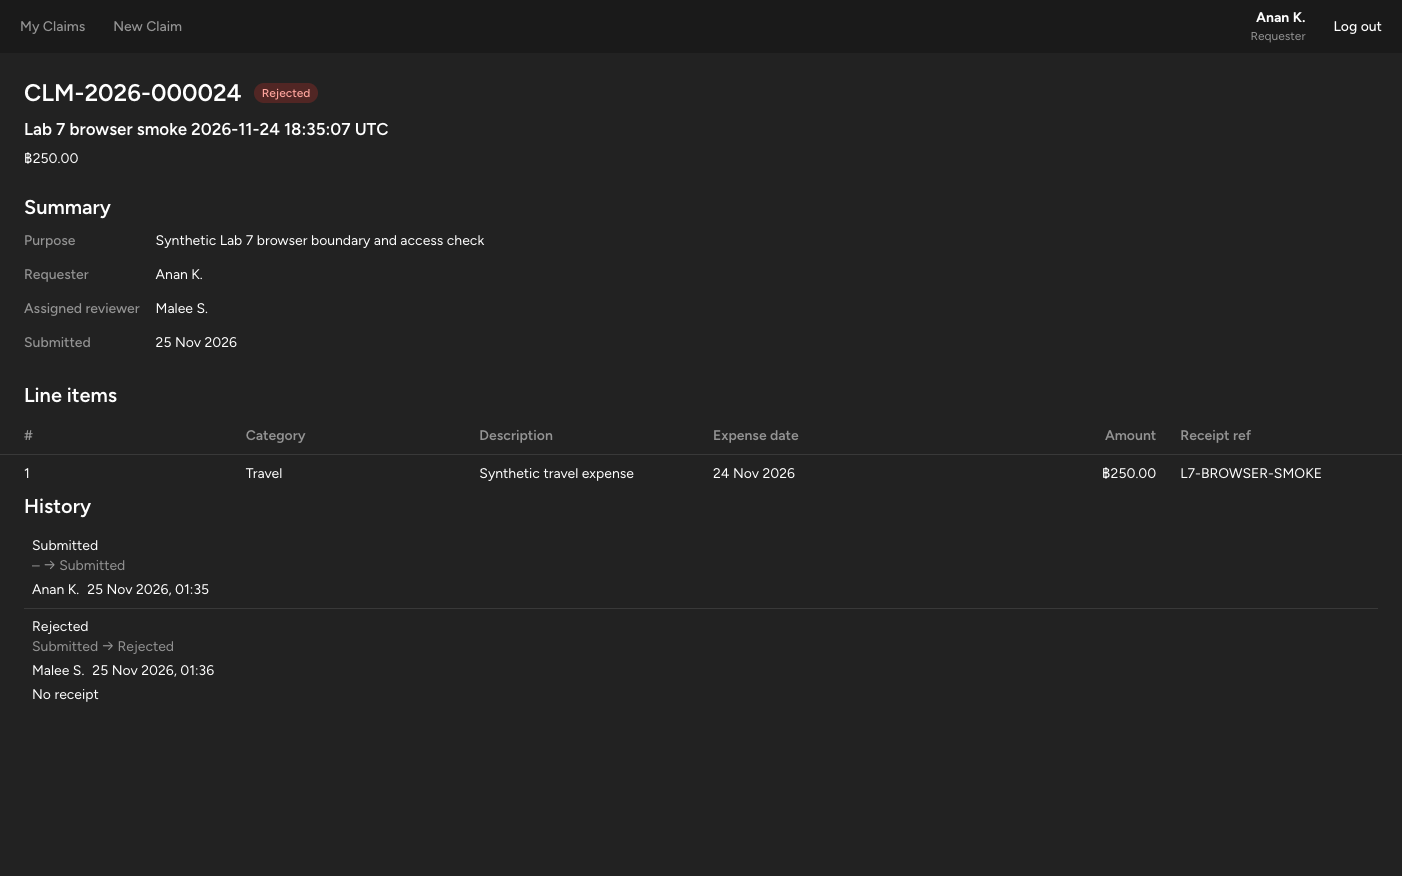
\includegraphics[width=0.96\linewidth,trim=0bp 156bp 0bp 0bp,clip]{figures/deploy/05-requester-history.png}
  \caption*{\textbf{B-08e.} The requester reopened the rejected claim and saw “No receipt” in history.}
\end{figure}

\reportpartend{B}

\reportpart{C}{Objective engineering metrics}
\label{ev:metrics}
All metrics are for the ClaimFlow repository. Dates use UTC in November 2026. The evidence snapshot was taken on 24 November at about 18:23, after the main release and deploy runs completed.

\begin{longtable}{@{}R{3.5cm}R{4.9cm}R{7.7cm}@{}}
\toprule
\textbf{Metric and value} & \textbf{Definition and window} & \textbf{Underlying evidence} \\ \midrule \endhead
C-01 \newline Completed Lab 7 requests \newline \textbf{1 completed} &
Count Issues with label \texttt{lab7} closed as completed from 22 Nov 00:00 through the 24 Nov snapshot. Excludes PRs, duplicates and cancellations. &
\issuelink{99} (L7/01), the only Issue in this cohort, closed as completed on 24 Nov at 17:48:07. Incorporated by release \prlink{106}. Neither a duplicate nor a cancellation. \\
C-02 \newline Merged maintenance PRs \newline \textbf{3 merged} &
Count merged PRs in the L7/01 release chain on 24 Nov. Scope is contract, implementation and main release. &
\prlink{101}: 16:18:19, \texttt{lab-7}, \texttt{124cf9a}. \newline
\prlink{105}: 17:31:06, \texttt{lab-7}, \texttt{8b660a1}. \newline
\prlink{106}: 17:48:05, \texttt{main}, \texttt{c32e645}. \\
C-03 \newline Release web tests \newline \textbf{139 passed, 0 failed, 0 skipped} &
Count test cases in one web coverage run on released main, 24 Nov 17:48:25--17:48:50. &
Main CI \runlink{45452555188}, \texttt{c32e645}, web job 138653270239. Summary shows 139 of 139 tests in 17 of 17 files. Command and excerpt in B-05 on p.~\pageref{ev:release}. \\
C-04 \newline Tracked Sprint 1 UAT defects \newline \textbf{0 open, 2 resolved} &
24 Nov snapshot of ClaimFlow's \texttt{uat}-labelled Sprint 1 findings. Resolved means a completed Issue plus passing partner retest. &
\issuelink{86} (minor, whitespace-only title/purpose), closed 22 Nov at 08:26:45. \newline
\issuelink{87} (major, duplicate Submit), closed 22 Nov at 08:26:39. \newline
Both fixes were on \texttt{bb5a0d1}, retested for Lab 6 and accepted at 11:27 on 22 Nov. This is a tracked-issue snapshot. \\
C-05 \newline Main workflow outcomes \newline \textbf{2 success, 0 fail, 0 cancelled} &
Count \texttt{CI} and \texttt{Deploy demo} runs created on \texttt{main} on 24 Nov through the snapshot. This scope excludes PR CI and earlier pushes. &
\runlink{45452555188}: CI push at 17:48:08, success, attempt 1. \newline
\runlink{45453647851}: Deploy demo at 17:54:12, success, attempt 1. Both at \texttt{c32e645}. \\
\bottomrule
\end{longtable}

\textbf{Action from the metrics.}
Both main workflows succeeded and the release web run passed 139 cases. The deploy workflow verifies service health, so all four authenticated boundary and access checks required a separate run. Before Final Delivery, the release owner (\texttt{beambeambeam}, proposed) should add a gated synthetic post-deploy smoke for those four checks. Keep credentials in managed secrets, emit only status and state summaries, and have \texttt{Kiatisakk} review the evidence before sign-off.

\reportpartend{C}

\reportpart{D}{Release readiness and retrospective}
\partsection{D-01}{Readiness checklist}
\label{ev:ready}
\textbf{READY for maintained Sprint 1 functionality on \texttt{v0.1.0.0} / \revision{}.}
The release passed CI and public smoke. The live probes exercised login (F-01), synthetic claim submission (F-02), My Claims and requester history (F-03), and the rejection boundary and access checks (F-04) in B-07 and B-08. Only the local F-04 E2E journeys were rerun for this change. E2E runs on a local seeded stack outside CI, per \prlink{96}. The ready decision combines these selected checks with Lab 6 acceptance and the release regression suites.

\begin{longtable}{@{}R{4cm}R{12.1cm}@{}}
\toprule
\textbf{Gate} & \textbf{Evidence and disposition} \\ \midrule \endhead
Version and deploy & \textbf{Pass}. Main and release tag resolve to \releaseSHA{}. Deploy demo \runlink{45453647851} served \revision{} with 100\% traffic and passed all public smoke checks. The live version and smoke were independently rechecked in this report session (B-06). \\
Automated regression & \textbf{Pass}. Main web had 139 passes and main Go had 300 passes, both with 0 failures and 0 skips. Go coverage was 100\% (785/785). Local named F-04 cases and both seeded E2E journeys passed. Earlier concurrent web runs timed out in F01-TEST-20. The isolated retry run and released CI passed. Pre-merge release jobs were skipped by design (B-04, B-05). \\
Selected deployed behavior & \textbf{Pass}. 4 authenticated HTTP checks and 6 live browser checks passed with synthetic users. The first HTTP probe was rerun after correcting its response assertion. Lab 6 partner acceptance is historical (A-01, B-07, B-08). \\
Defects by severity & \textbf{0 open in tracked Sprint 1 UAT}. Major \#87 and minor \#86 were fixed, retested and closed in Lab 6 (C-04). No new product defect surfaced in the Lab 7 checks. \\
Configuration and secrets & \textbf{Pass for release configuration}. The release used the existing Lab 5 workload identity and deploy pipeline. No schema, service setting, or secret change was required for BR-04. Demo credentials stay in private course handoff. Students should confirm grader access before submission. \\
Documentation and run instructions & \textbf{Pass}. Versioned SRS, F-04, System SDS and STS, traceability and OpenAPI agree on the new rule. Use the repository README for local setup and B-06 to B-08 for release and behavior checks. \\
\bottomrule
\end{longtable}

\textbf{Deferred engineering work.}
\begin{longtable}{@{}R{3.5cm}R{6.1cm}R{2cm}R{4cm}@{}}
\toprule
\textbf{Item} & \textbf{Impact} & \textbf{Priority} & \textbf{Disposition} \\ \midrule \endhead
Authenticated deploy tests run on demand & Green pipeline smoke cannot catch drift in boundary or access behavior. & High & Before Final Delivery, add the gated synthetic smoke in Part C. \\
Trim/count logic in Go and web & Separate implementations depend on shared semantics. Divergence can block a valid reason in the dialog. & Medium & Keep the boundary vectors in both test layers. Proposed reviewer \texttt{Kiatisakk} checks parity when a later decision path reuses the rule. \\
F01-TEST-20 login timeouts under concurrent load & Local web checks timed out during login. The isolated run passed with \texttt{--retry=2}, which can mask intermittent failures. & Medium & Proposed owner \texttt{beambeambeam} reproduces under load and reruns the isolated suite without retries before Final Delivery. \\
\bottomrule
\end{longtable}

\clearpage
\partsection{D-02}{Retrospective}
\textbf{What helped?}
The revised STS made the 9/10 boundary testable before changing the service. The same checks turned green and verified that refusal left history and version intact.

\textbf{What hurt?}
Implementation started while the OpenAPI review was pending, so sequence evidence needed a follow-up. Running suites concurrently also caused login timeouts and made the local web result harder to interpret.

\textbf{What will change?}
Record contract approval before implementation and run the web coverage check in isolation. Before Final Delivery, make the four authenticated demo checks part of the release evidence.

\partsection{D-03}{Contributions and AI use}
\begin{longtable}{@{}R{4cm}R{12.1cm}@{}}
\toprule
\textbf{Contributor} & \textbf{Work on the maintenance change} \\ \midrule \endhead
\texttt{Kiatisakk} & Reviewed the request baseline and scope in \#99. Authored and revised Part A in \#101. Reviewed OpenAPI, generation, tests and evidence on \#105, requested fixes to the record, then approved \#105 and \#106. \\
\texttt{beambeambeam} & Opened and updated \#99 and recorded the course waiver. Reviewed and approved Part A in \#101. Authored the OpenAPI, test, implementation and verification changes in \#105 and authored release PR \#106. \\
Pair work & Both students planned the change, drafted the specification, and prepared the ticket together. \#105 records Part B as individual work with teammate review. \\
\bottomrule
\end{longtable}

\textbf{AI-use declaration.}
We both used AI to plan Lab 7. We used \texttt{grill-with-docs} to examine the proposed change against the project documentation, then \texttt{to-spec} to draft the specification, and \texttt{to-ticket} to draft the GitHub issue. We also used AI assistance during implementation and used \texttt{code-review} to help review changes. AI assisted with release documentation, report preparation, and the HTTP and browser evidence in B-06 to B-08. Both students should confirm this declaration before submission.

\textbf{Known limitations.}
Independent partner UAT evidence comes from the accepted Lab 6 release. The waiver is documented through the team's issue comment. Deployment evidence is pinned to \texttt{c32e645} and \revision{}. Later main deployments, including a Sprint 2 release via \prlink{102}, may change what the live URL serves. Historical Lab 6 data and the two synthetic Lab 7 claims stay in the demo. The team should confirm private grader access and deployment availability through grading.

\reportpartend{D}

\end{document}
